% Nguồn SGK Toán 9 Tập hai — Bài 21, trang 25--27:
% https://cdn3.olm.vn/upload/thuvienso/4491669493-page-25-1771844542977.png
% https://cdn3.olm.vn/upload/thuvienso/4491669493-page-26-1771844543289.png
% https://cdn3.olm.vn/upload/thuvienso/4491669493-page-27-1771844543621.png
% Authority: https://olm.vn/thu-vien-so/doc-sach/sach.4491669493.4491669493
%
% Nguồn SBT Toán 9 Tập hai — Bài 21, PDF trang 17--18:
% SBT TOÁN 9 TẬP 2.pdf (Project Sources)
% SHA-256: 5ff01fd213d1adc75f9c54b4408d6a9642a4d8038e685040efef3311a196196c
% Phạm vi SBT: 6.25--6.32; PDF trang 18 chỉ lấy phần trước ÔN TẬP CHƯƠNG VI.

\section{Giải bài toán bằng cách lập phương trình}

\begin{lesson}
    \subsection{Kiến thức trọng tâm}

    \begin{center}
    \begin{tblr}{
        width=\linewidth,
        colspec={X[2,l] X[5,l]},
        cells={valign=t},
        row{1}={font=\bfseries, halign=c}
    }
        Khái niệm, thuật ngữ & Kiến thức, kĩ năng \\
        Giải bài toán bằng cách lập phương trình & Giải quyết một số vấn đề thực tiễn gắn với phương trình bậc hai một ẩn.
    \end{tblr}
    \end{center}

    Bác Lan gửi tiết kiệm 100 triệu đồng vào ngân hàng với kì hạn 12 tháng theo thể thức lãi kép. Sau năm thứ nhất, do chưa có nhu cầu sử dụng nên bác Lan không rút tiền ra mà tiếp tục gửi 12 tháng nữa, với lãi suất như cũ. Sau hai năm bác Lan rút tiền ra thì nhận được 118,81 triệu đồng cả vốn lẫn lãi. Hỏi lãi suất gửi tiết kiệm là bao nhiêu?

    \subsubsection{Giải bài toán bằng cách lập phương trình}

    Xét bài toán ở \textit{tình huống mở đầu}.

    \textbf{HĐ1} Gọi $x$ là lãi suất gửi tiết kiệm của bác Lan ($x$ được cho dưới dạng số thập phân). Hãy biểu thị số tiền thu được (cả vốn lẫn lãi) của bác Lan sau kì gửi thứ nhất theo $x$.

    \answerline
    \answerline

    \textbf{HĐ2} Hết kì gửi thứ nhất, bác Lan không rút tiền ra mà tiếp tục gửi tiết kiệm kì thứ hai với lãi suất như cũ. Hãy biểu thị số tiền thu được (cả vốn lẫn lãi) của bác Lan sau kì gửi thứ hai theo $x$.

    \answerline
    \answerline

    \textbf{HĐ3} Dựa vào đề bài, viết phương trình ẩn $x$ thu được và giải phương trình này để tìm $x$. Từ đó, trả lời câu hỏi trong \textit{tình huống mở đầu}.

    \answerline
    \answerline
    \answerline

    \textbf{Nhận xét.} Các bước giải một bài toán bằng cách lập phương trình:

    \textit{Bước 1.} Lập phương trình:
    \begin{itemize}
        \item Chọn ẩn số và đặt điều kiện thích hợp cho ẩn số.
        \item Biểu diễn các đại lượng chưa biết theo ẩn và các đại lượng đã biết.
        \item Lập phương trình biểu thị mối quan hệ giữa các đại lượng.
    \end{itemize}

    \textit{Bước 2.} Giải phương trình.

    \textit{Bước 3.} Trả lời: Kiểm tra xem trong các nghiệm của phương trình, nghiệm nào thoả mãn điều kiện của ẩn, nghiệm nào không, rồi kết luận.

    \textbf{Ví dụ 1}

    Một sân bóng đá 7 người có chiều rộng nhỏ hơn chiều dài 30 m và có diện tích bằng $1\,800\,\text{m}^2$. Tính chiều dài và chiều rộng của sân bóng đó.

    \textbf{Giải}

    Gọi $x$ (m) là chiều rộng của sân bóng. Điều kiện: $x>0$.

    Khi đó, chiều dài của sân bóng là $x+30$ (m).

    Theo đề bài, ta có phương trình:
    \[
        x(x+30)=1\,800\ \text{ hay }\ x^2+30x-1\,800=0.
    \]
    Ta có: $\Delta'=15^2+1\,800=2\,025$, $\sqrt{\Delta'}=45$.

    Suy ra phương trình có hai nghiệm phân biệt:
    \[
        x_1=\dfrac{-15-45}{1}=-60\ (\text{loại});\qquad
        x_2=\dfrac{-15+45}{1}=30\ (\text{thoả mãn điều kiện}).
    \]
    Vậy sân bóng có chiều dài 60 m và chiều rộng 30 m.

    \textbf{Ví dụ 2}

    Khoảng cách giữa hai bến sông $A$ và $B$ là 36 km. Một tàu du lịch đi từ bến $A$ đến bến $B$, nghỉ 30 phút ở bến $B$ rồi quay lại bến $A$. Thời gian kể từ lúc khởi hành đến khi về đến bến $A$ là 5,5 giờ. Hãy tìm vận tốc thực của tàu du lịch (tức là vận tốc của tàu khi nước yên lặng), biết rằng vận tốc của dòng nước là 3 km/h.

    \textbf{Giải}

    Gọi $x$ (km/h) là vận tốc thực của tàu du lịch. Vì vận tốc của dòng nước là 3 km/h nên phải có điều kiện $x>3$ để tàu có thể chạy ngược dòng.

    Vận tốc của tàu khi xuôi dòng là $x+3$ (km/h), thời gian để tàu đi xuôi dòng là $\dfrac{36}{x+3}$ (giờ).

    Vận tốc của tàu khi ngược dòng là $x-3$ (km/h), thời gian để tàu đi ngược dòng là $\dfrac{36}{x-3}$ (giờ).

    Thời gian tàu nghỉ tại bến $B$ là 30 phút = 0,5 giờ.

    Theo đề bài, ta có phương trình:
    \[
        \dfrac{36}{x+3}+0{,}5+\dfrac{36}{x-3}=5{,}5
        \ \text{hay}\ 
        \dfrac{36}{x+3}+\dfrac{36}{x-3}=5.
    \]
    Để giải phương trình này, ta quy đồng mẫu vế trái của phương trình:
    \[
        \dfrac{36(x-3)+36(x+3)}{(x+3)(x-3)}=5.
    \]
    Nhân cả hai vế của phương trình với $(x+3)(x-3)$ để khử mẫu, ta được phương trình bậc hai
    \[
        36(x-3)+36(x+3)=5(x+3)(x-3),\ \text{hay}\ 5x^2-72x-45=0.
    \]
    Ta có: $\Delta'=(-36)^2-5\cdot(-45)=1\,521$; $\sqrt{\Delta'}=\sqrt{1\,521}=39$.

    Suy ra phương trình có hai nghiệm phân biệt:
    \[
        x_1=\dfrac{36-39}{5}=-\dfrac{3}{5}\ (\text{loại});\qquad
        x_2=\dfrac{36+39}{5}=15\ (\text{thoả mãn điều kiện}).
    \]
    Vậy vận tốc thực của tàu du lịch là 15 km/h.

    \textbf{Luyện tập}

    Một đội xe gồm các xe tải cùng loại, cần phải chở 120 tấn hàng. Tuy nhiên khi làm việc, có hai xe phải điều chuyển đi nơi khác nên mỗi xe phải chở thêm 3 tấn hàng. Hỏi đội xe đó có bao nhiêu chiếc xe tải?

    \answerline
    \answerline
    \answerline
\end{lesson}

\begin{exercises}
    \subsection{Bài tập}

    \begin{questions}[resume=SGK]
        \item Một mảnh đất hình chữ nhật có diện tích $360\,\text{m}^2$. Nếu tăng chiều rộng 3 m và giảm chiều dài 4 m thì diện tích mảnh đất không đổi. Tìm các kích thước của mảnh đất đó.

        \answerline
        \answerline
        \answerline

        \item Sau hai năm, số dân của một thành phố tăng từ $1\,200\,000$ người lên $1\,452\,000$ người. Hỏi trung bình mỗi năm dân số của thành phố đó tăng bao nhiêu phần trăm?

        \answerline
        \answerline
        \answerline

        \item Một thanh sô cô la có dạng hình hộp chữ nhật với chiều dài 12 cm, chiều rộng 7 cm và độ dày 3 cm. Do giá nguyên liệu ca cao tăng nhưng vẫn muốn giữ nguyên giá bán nên nhà sản xuất quyết định giảm 10\% thể tích của mỗi thanh sô cô la. Để thực hiện việc này, nhà sản xuất dự định làm thanh sô cô la mới có cùng độ dày 3 cm như thanh cũ, nhưng chiều dài và chiều rộng sẽ giảm đi cùng một số centimét. Hỏi kích thước của thanh sô cô la mới là bao nhiêu (làm tròn kết quả đến hàng phần trăm của cm)?

        \answerline
        \answerline
        \answerline

        \item Một máy bay khởi hành từ Hà Nội vào Thành phố Hồ Chí Minh, sau đó nghỉ 96 phút và tiếp tục bay về Hà Nội với vận tốc lớn hơn vận tốc lúc đi là 100 km/h. Tổng thời gian của cả hành trình, kể từ khi xuất phát từ Hà Nội đến khi quay về Hà Nội là 6 giờ. Tính vận tốc của máy bay lúc đi, biết quãng đường bay Hà Nội – Thành phố Hồ Chí Minh dài khoảng $1\,200$ km.

        \answerline
        \answerline
        \answerline

        \item Một ô tô khách khởi hành từ Hà Nội đi Hải Phòng. Sau đó 30 phút, một ô tô con xuất phát từ cùng địa điểm ở Hà Nội và cũng đi về Hải Phòng trên cùng tuyến đường, với vận tốc lớn hơn vận tốc của ô tô khách là 20 km/h. Hai xe đến cùng một địa điểm ở Hải Phòng tại cùng một thời điểm. Hãy tính vận tốc của mỗi ô tô, biết rằng quãng đường Hà Nội – Hải Phòng dài khoảng 120 km.

        \answerline
        \answerline
        \answerline

        \item Một xưởng may phải may $1\,500$ chiếc áo trong thời gian quy định. Để hoàn thành sớm kế hoạch, mỗi ngày xưởng đã may được nhiều hơn 10 chiếc áo so với số áo phải may trong một ngày theo kế hoạch. Do đó, ba ngày trước khi hết thời hạn, xưởng đã may được $1\,320$ áo. Hỏi theo kế hoạch, mỗi ngày xưởng đó phải may xong bao nhiêu chiếc áo?

        \answerline
        \answerline
        \answerline
    \end{questions}
\end{exercises}

\begin{practice}
    \subsection{Luyện tập}

    \begin{questions}[resume=SBT]
        \item Một bức ảnh hình chữ nhật có chiều rộng 8 cm và chiều dài 12 cm. Bức ảnh được phóng to bằng cách tăng chiều dài và chiều rộng thêm một đoạn bằng nhau để tăng gấp đôi diện tích của bức ảnh. Tìm kích thước của bức ảnh mới.

        \answerline
        \answerline
        \answerline

        \item \textit{Hình chữ nhật vàng} là hình chữ nhật có thể chia thành một hình vuông và hình chữ nhật thứ hai có các kích thước tỉ lệ với các kích thước tương ứng của hình chữ nhật ban đầu (với cùng hệ số tỉ lệ). Tỉ số $x$ giữa chiều dài và chiều rộng của hình chữ nhật vàng được gọi là \textit{tỉ lệ vàng}.

        \begin{center}
            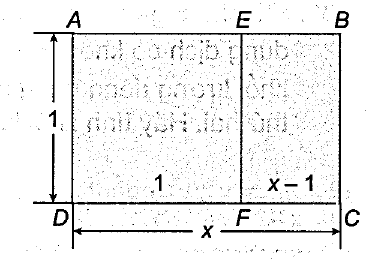
\includegraphics[width=0.46\linewidth]{content/chapter-01/figures/lesson-21-sbt-6-26.png}
        \end{center}

        \begin{questions}
            \item Tìm tỉ số giữa chiều dài và chiều rộng của hình chữ nhật $ABCD$ và hình chữ nhật $EBCF$.

            \answerline
            \answerline
            \item Tìm giá trị chính xác của tỉ lệ vàng bằng cách đặt hai tỉ số ở câu a bằng nhau rồi tìm $x$.

            \answerline
            \answerline
        \end{questions}

        \item Hai chiếc máy bay khởi hành đồng thời từ một sân bay, một chiếc bay theo hướng bắc và chiếc kia bay theo hướng đông (xem hình bên). Chiếc máy bay đi về hướng bắc đang bay nhanh hơn 50 dặm một giờ so với chiếc máy bay đi về hướng đông. Sau 3 giờ, hai máy bay cách nhau $2\,440$ dặm. Tìm vận tốc của mỗi máy bay.

        \begin{center}
            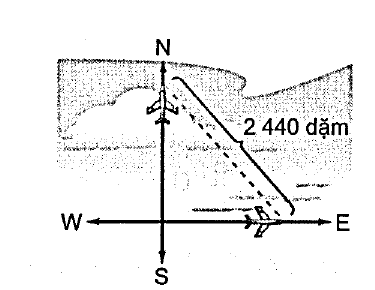
\includegraphics[width=0.36\linewidth]{content/chapter-01/figures/lesson-21-sbt-6-27.png}
        \end{center}

        \answerline
        \answerline
        \answerline

        \item Một phòng họp lúc đầu có một số dãy ghế với tổng cộng 40 chỗ ngồi. Do phải sắp xếp 55 chỗ ngồi cho một cuộc họp nên người ta kê thêm một dãy ghế và mỗi dãy ghế xếp thêm một chỗ ngồi. Hỏi lúc đầu có mấy dãy ghế trong phòng họp đó?

        \answerline
        \answerline
        \answerline

        \item Hai anh em Hùng và Nam được mẹ giao nhiệm vụ dọn nhà. Nếu cả hai anh em cùng làm thì mất $2\dfrac{2}{5}$ giờ để dọn xong nhà. Nếu làm một mình thì tổng cộng thời gian của cả hai anh em để dọn xong là 10 giờ. Hỏi mỗi người cần bao nhiêu thời gian để dọn xong nhà khi làm một mình? (Biết rằng Hùng làm nhanh hơn Nam).

        \answerline
        \answerline
        \answerline

        \item Một cái hộp không có nắp được làm từ mảnh bìa hình chữ nhật có kích thước 30 cm $\times$ 40 cm bằng cách cắt ở bốn góc của mảnh bìa bốn hình vuông bằng nhau. Diện tích phần đáy hộp là $336\,\text{cm}^2$. Tính độ dài mỗi cạnh hình vuông cắt ra ở bốn góc.

        \answerline
        \answerline
        \answerline

        \item Một người đi xe máy từ tỉnh $A$ đến tỉnh $B$. Sau đó 16 phút có một ô tô đi từ $B$ về $A$ với vận tốc lớn hơn vận tốc của xe máy là 15 km/h. Xe máy gặp ô tô ở một địa điểm cách $B$ 24 km. Tính vận tốc của ô tô, biết rằng quãng đường $AB$ dài 54 km.

        \answerline
        \answerline
        \answerline

        \item Khi pha 8 gam chất lỏng thứ nhất với 6 gam chất lỏng thứ hai thì được một dung dịch có khối lượng riêng là $0{,}7\,\text{g/cm}^3$. Biết rằng chất lỏng thứ nhất có khối lượng riêng nặng hơn $0{,}2\,\text{g/cm}^3$ so với khối lượng riêng của chất lỏng thứ hai. Hãy tính khối lượng riêng của mỗi chất lỏng ban đầu.

        \answerline
        \answerline
        \answerline
    \end{questions}
\end{practice}
